\section{Zadanie 5}

\subsection{Charakterystyka algorytmu Clenshawa}

Algorytm Clenshawa to efektywna metoda obliczania wartości wielomianu w postaci Czebyszewa przy złożoności \( O(n) \). W porównaniu ze standardowym sposobem wyznaczania wartości wielomianów, algorytm ten jest zoptymalizowany do przetwarzania ich w postaci rekurencyjnej, co prowadzi do znacznego przyspieszenia obliczeń.

W ramach eksperymentu porównano szybkość działania algorytmu Clenshawa z klasycznym sposobem obliczania wielomianów Czebyszewa. Wyniki przedstawiono na wykresie, który uwzględnia średni czas wykonania dla obu metod. Ustawienia jak w zadaniu 1.

\subsection{Wyniki i wnioski}

\begin{center}
% Wykres czasu porównania Clenshawa i metody standardowej
\textbf{Średni czas dla metody Clenshawa:} \( 0.000578 \pm 0.000324 \)  
\textbf{Średni czas dla metody standardowej:} \( 0.000692 \pm 0.000393 \)  
\textbf{Przyspieszenie:} \( 1.20 \times \pm 0.03 \times \)
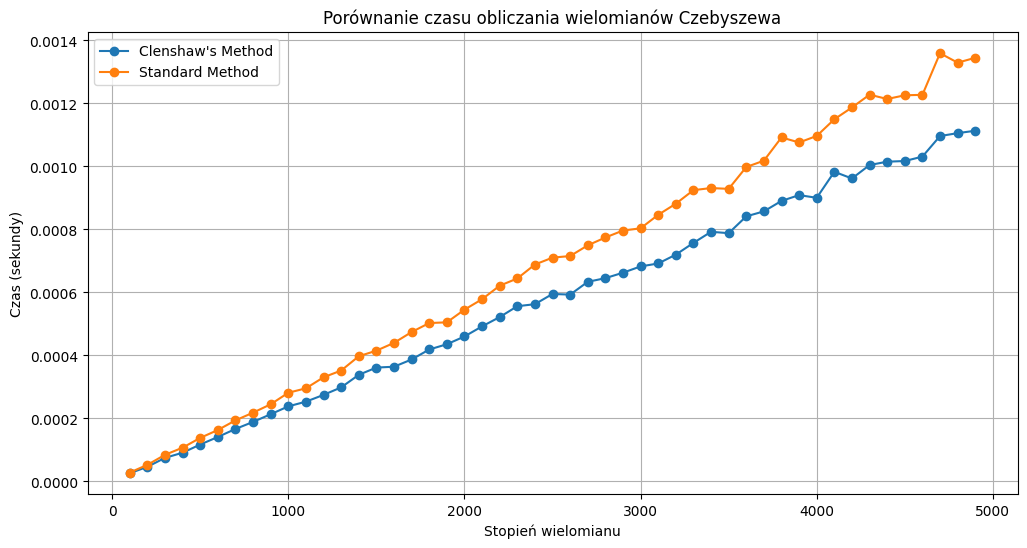
\includegraphics[width=\textwidth]{wykresy/zadanie 4/czebyszew_5000.png}
\end{center}

\textbf{Wnioski:}
\begin{itemize}
    \item \textbf{Szybkość metody Clenshawa:} Algorytm Clenshawa wykazuje wyraźną przewagę nad standardową metodą liczenia wielomianów Czebyszewa, osiągając średnio 1.20x szybsze wykonanie.
    \item \textbf{Porównanie z Hornerem:} Metoda Clenshawa jest bliska optymalnemu czasowi obliczeń znanemu z algorytmu Hornera, który jest specjalnym przypadkiem dla wielomianów Czebyszewa.
    \item \textbf{Stabilność czasów:} W odróżnieniu od algorytmu Hornera, metoda Clenshawa nie wykazuje wahań w czasie wykonania, co świadczy o jej większej stabilności numerycznej.
\end{itemize}
